%----------------------------------------------------------------
%
%  File    :  thesis-tech.tex
%
%  Author  :  Eva Rott, TU Graz, Austria
% 
%  Created :  14 May 2017
% 
%  Changed :  16 May 2017
% 
%----------------------------------------------------------------


\chapter{Reordering}
\label{chap:reordering}

Reordering describes the process of either moving nodes in a graph or moving rows or columns in a matrix. There are two types of reordering: manual and automatic. The former is done by the user of a program. The latter is computed by a software tool using its implemented algorithms. This survey focuses on automatic reordering.

The information used as input for the reordering algorithms can either be the node label, node in or out degree or clustering data. The mentioned information sources are not a complete list of available reordering input data. However, they were found in the tested programs and are described in more detail in the following sections.


\section{Reordering Using Node Label}
\label{sec:reordering_label}
The data used for this example describes a number of functions of a program connected corresponding to their control flow. Figure \ref{fig:reordering_example_graph} shows the directed graph with the functions as nodes; figure \ref{fig:reordering_example_matrix} shows the unsorted matrix representation of the graph. The result of reordering the matrix based on alphabetic label name order can be seen in \ref{fig:reordering_example_label}.

\begin{figure}[tp]
  \centering
  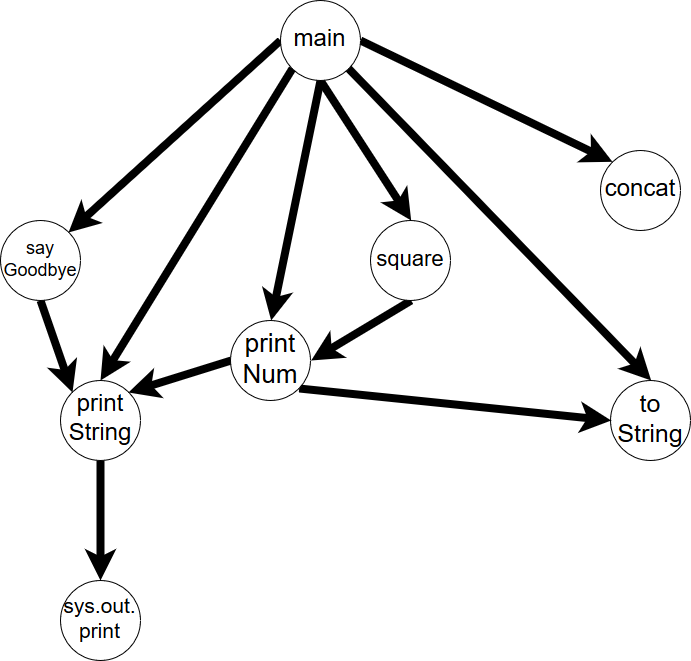
\includegraphics[keepaspectratio,width=\hsize,height=\halfh]
  {images/Reordering_Example_graph.png}

  \caption[Directed Graph of Sample Data]{
  The nodes are functions in a program connected corresponding to control flow.
  \imgcredit{Image created by an author of this thesis using \url{www.draw.io}.}
  }
  \label{fig:reordering_example_graph}
\end{figure}

\begin{figure}[tp]
  \centering
  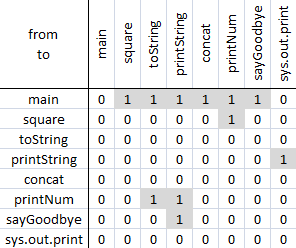
\includegraphics[scale=0.9]
  {images/Reordering_Example_matrix.png}
  
  \caption[Matrix Representation of Sample Data]{
  This is the matrix corresponding to \ref{fig:reordering_example_graph}. Function callers are marked in the columns and function callees in the rows.
  \imgcredit{Image created by an author of this thesis using Microsoft Excel.}
  }
  \label{fig:reordering_example_matrix}
\end{figure}

\begin{figure}[tp]
  \centering
  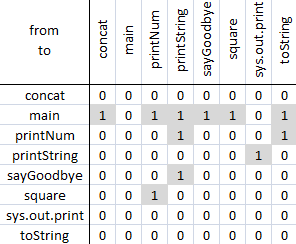
\includegraphics[scale=0.9]
  {images/Reordering_Example_label.png}
  
  \caption[Reordered Matrix Based on Labels]{
  The original matrix is reordered using alphabetic sorting of the labels.
  \imgcredit{Image created by an author of this thesis using Microsoft Excel.}
  }
  \label{fig:reordering_example_label}
\end{figure}


\section{Reordering Using Node Out Degree}
The data used for this example is the same as in \ref{sec:reordering_label}. Figure \ref{fig:reordering_example_degree} shows a reordered matrix based on ascending order of node in and out degree. The function with the largest number of incoming links is the rightmost column and the node with the largest number of outgoing links the lowermost row of the matrix.

\begin{figure}[tp]
  \centering
  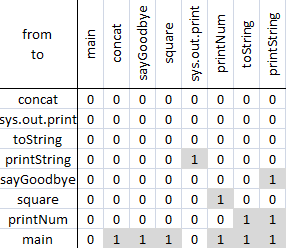
\includegraphics[scale=0.9]
  {images/Reordering_Example_degree.png}
  
  \caption[Reordered Matrix Based on Node Degree]{
  The original matrix is reordered using information about the degree of the nodes. The columns are sorted corresponding to their out degree and the rows to in degree.
  \imgcredit{Image created by an author of this thesis using Microsoft Excel.}
  }
  \label{fig:reordering_example_degree}
\end{figure}


\section{Reordering Using Node Clustering}
As node clustering needs to be computed first, this type of reordering is explained in an example taken from the program Nodetrix. Displayed in figure \ref{fig:reordering_nodetrix_cluster} is the graph with the clustered nodes marked in different colors, and sub-matrices for some of the ordered clusters.

\begin{figure}[tp]
  \centering
  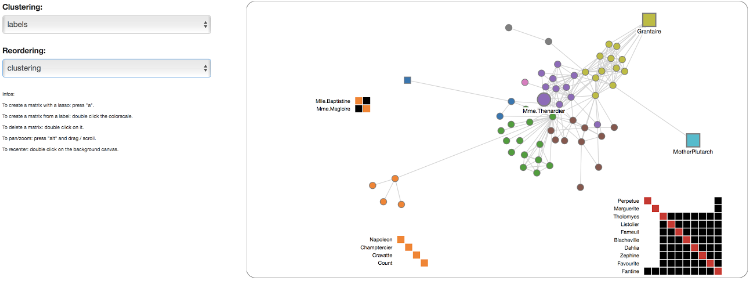
\includegraphics[keepaspectratio,width=\hsize,height=\halfh]
  {images/Reordering_NodeTrix_cluster.png}
  
  \caption[Reordered Matrix Based on Clustering]{
  The original matrix is reordered using clustering information which is computed based on node labels.
  \imgcredit{Screenshot created by an author of this thesis using Nodetrix. \citep[1302-1309]{henry-nodetrix-2007}.}
  }
  \label{fig:reordering_nodetrix_cluster}
\end{figure}
